\documentclass{article}

\usepackage[margin=1in]{geometry}
\usepackage{minted}
\usepackage{amsmath}
\usepackage{amssymb}
\usepackage{graphicx}
\usepackage{subcaption}
%\usepackage{float}
\usepackage{xcolor}
\usepackage{setspace}
\usepackage{hyperref}
\usepackage[backend=biber]{biblatex}

\bibliography{progress-report.bib}
\doublespacing

\title{Final Project Progress Report}
\author{Leanna Calla\\Michael Stergianis}
\date{\today}

\begin{document}
\maketitle

\section{Introduction}
We will be examining the imaging application of Image and Video super
resolution. This application uses some ideas explored
in class and has various real world applications. 
\section{Interpolation}
\label{sec:interpolation}
Much of work in super resolution has to do with interpolation.  There
are many interpolation schemes that can be used in order to increase
the resolution of images. This section will briefly describe a few
interpolation schemes of note.
%
\subsection{Bilinear Interpolation}
\label{subsec:bilinear}
Bilinear interpolation is the process of supposing a subpixel
surrounded by four real pixels and interpolating linearly between the
four pixels to find the subpixel.
%
%
\section{Uses}
\label{sec:uses}

Super resolution is incredibly useful. As noted in
\cite{Yang2010ImageSH}, there are a few major areas where super
resolution particularly useful.
\subsection{Surveillance Video}
As noted in \cite{Yang2010ImageSH}, super resolution has applications
which involve the manipulations of surveillance videos. One may be
required to freeze a video
to zoom into a specific area. This may help to look at things like faces or license plates.
\subsection{Remote Sensing}
\cite{Li} discusses the applications of super resolution on satellite
images. The figures below give an example of the improvements that can
be seen by applying a Wiener filter to a low resolution image. These
figures come from \cite{Li}.    
\begin{figure}[H]
  \centering
  \begin{subfigure}[b]{0.5\textwidth}
    \centering
  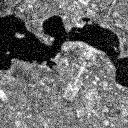
\includegraphics[width= 0.4\linewidth]{LR-satellite.png}
  \caption{\label{fig:label} Satellite low res }
\end{subfigure}%
\begin{subfigure}[b]{0.5\textwidth}
  \centering
  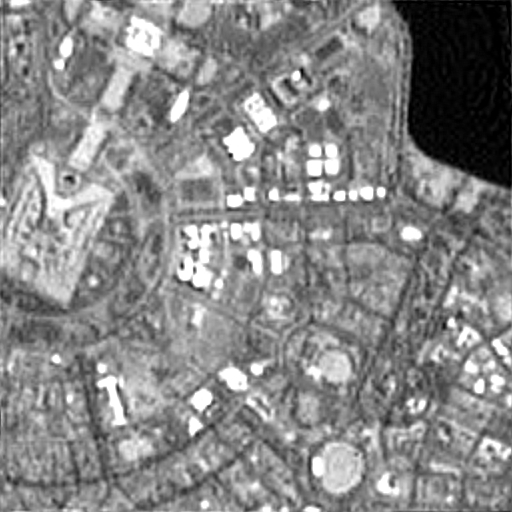
\includegraphics[width = 0.4\linewidth]{SR-satellite.png}
  \caption{\label{fig:label} Satellite super res }
  \end{subfigure}
\end{figure}
Satellite image improvement also has applications for forestry and
agriculture, as noted in \cite{LiSatellite}.

\subsection{Medical Imaging}
Super resolution has applications in Medical Imaging such as improving
the quality of MRI images. \cite{Peled} notes that the quality of the resolution of
an MRI has limitations such as the imaging time and any
movement of the patient. The diffusion-sensitized echo-planar imaging
technique, \cite{Peled}, acquires the image in shot, avoiding phase problems. Some
limitations do remain for things like brain images.  


\subsection{Multiple Image Resolution}
Low resolution images can be combined into one higher resolution
image. This is known as multiple image super resolution. In
\cite{CapelMulti}, we see multiple images can be used as training
data. This paper explores the use of training images
to set the constraints in the maximum likelihood estimation. This work
is applied to images of faces in \cite{CapelMulti}.
 
\section{Future Work}
\label{sec:future}
As seen in section \ref{sec:uses}, there are many practical
applications of super resolution that are of great benefit to various
disciplines and areas of industry. We would like to explore this topic
further in order to produce some working code that can be applied to a low
resolution image. We plan to proceed and accomplish the following
tasks:
\begin{itemize}
\item Find databases of low resolution images for the
  above listed applications
  \item Create low resolution images by adding noise
  \item Explore and implement interpolation techniques to produce
    super resolution images
    \item compare the qualitative differences of low and super
      resolution images. The following are noted in \cite{CapelMulti}
      \begin{itemize}
      \item blur
      \item  noise
      \item geometric warping
        
        \end{itemize}
      \item compare the quantitative differences of the images by
        tracking statistics
        \item Obtain statistics by comparing a produced high resolution image with
        the ground truth image 
\end{itemize}


\newpage
% Bibliography
\printbibliography
\end{document}
